\documentclass[runningheads,a4paper]{llncs}

\usepackage{amssymb}
\usepackage{amsmath}
\usepackage{subfig}

\usepackage{graphicx}
\usepackage{cite}
\usepackage{url}
\urldef{\mails}\path|{yang.deng, zhonghong.ou, antti.yla-jaaski}@aalto.fi|
\newcommand{\keywords}[1]{\par\addvspace\baselineskip
\noindent\keywordname\enspace\ignorespaces#1}

\begin{document}

\mainmatter

\title{Adaptive Packet Size Control for \\Bulk Data Transmission in IPv6 over\\Networks of Resource Constrained Nodes}
\titlerunning{Adaptive Packet Size Control for Bulk Data Transmission in 6lo}

\author{Yang Deng\and Zhonghong Ou\and Antti Yl\"a-J\"a\"aski}
\authorrunning{Y.Deng et al.}

\institute{Aalto University, Espoo, Finland\\ \mails}

\maketitle

\begin{abstract}
Conventional transmission in IPv6 over Networks of Resource Constrained Nodes favours fixed-size packet and results in low network performance when bulk data transmission is required by applications, for example firmware updating. To tackle this problem, we firstly investigate the performance of bulk data transmission through large packets and obtain two important observations. Then we propose an adaptive mechanism to dynamically adjust the packet size based on network conditions. We implement the mechanism on Contiki OS and evaluate it through a series of experiments in Cooja. Experimental results demonstrate that our adaptive mechanism outperforms Contiki standard implementation in terms of reliability and goodput in various network conditions.

\keywords{6lo, Bulk Data Transmission, Packet Size Control}
\end{abstract}

\section{Introduction}
IPv6 over Networks of Resource-constrained Nodes~(6lo) is a network that provides IPv6 connectivity over constrained nodes such as sensors or actuators. It has an adaptation layer to deal with the mappings between IPv6 packet and link frame (hereafter referred to as packet and frame respectively). Conventionally, when data are transmitted in 6lo, they are firstly encapsulated into a fixed-size packet and then header compression is applied to reduce the packet size. If the compressed packet fits into a single frame it will be sent directly; otherwise fragmentation-reassembly mechanism (hereafter referred to as 6lo fragmentation) is invoked. The value of the fixed-size is preconfigured empirically (e.g. 140 for IEEE 802.15.4 in Contiki). As RFC4944~\cite{rfc4944} pointed out, in links with a small maximum transmission unit (MTU) value, this conventional transmission works ordinarily with two assumptions that (i) most applications will not use large packets and (ii) application payload is relatively small. Nevertheless, there are scenarios where these conditions do not hold. Considering the firmware updating on-the-fly or massive data exchanging between nodes, both of them involve bulk data transmission for which 6lo conventional transmission is not suitable due to low network performance.

In order to improve the 6lo performance of bulk data transmission, we present an adaptive mechanism that adjusts the packet size based on network conditions and utilizes 6lo fragmentation (totally different from IP fragmentation) to send large packets. We implement the mechanism on Contiki OS and evaluate it through a series of experiments in Cooja. Overall, our work makes the following three key contributions:
\begin{itemize}
\item We investigate the performance of bulk data transmission in 6lo through large packets and obtain two important observations.
\item We present the design, implementation and evaluation of adaptive mechanism suitable for bulk data transmission in 6lo.
\item We show that our adaptive mechanism is able to provide better reliability and higher goodput than Contiki standard implementation in various network conditions.
\end{itemize}

\section{Related Work}
Before IPv6 is introduced to Wireless Sensor Network (WSN), packet size optimization for WSN has been studied extensively in literature. Modiano~et~al. develop a Markov chain model to analyse the channel then perform a maximum likelihood approach to estimate the frame size~\cite{Modi1999}. And Sankarasubramaniam~et~al. use energy-efficiency as the optimization object to determine the best frame size based on a set of radio and channel parameters~\cite{Sank2003}. The work from~\cite{Vura2008} discusses the cross-layer solutions to set the frame size for different environments like underwater and underground networks. All of these studies try to find a fixed size that the network uses. There is another thread of research work that suggests to use adaptive approaches. Jelenkovi\'{c}~et~al. design an algorithm to divide the frame into several small chunks to fit the available channel periods~\cite{Jele2008}. Dong's work~\cite{Dong2010} follows a similar idea where small chunks can be reassembled into a bigger frame. Nonetheless, the solutions mentioned above are not suitable for 6lo as they only work at link layer and are limited to a certain type of link. 6lo might run above different types of links and thus a solution working at IP layer is beneficial, which is the main contribution of this paper.

\section{Mechanism}

\subsection{Overview}\label{sec:ov}
Our motivation comes from the fact that bulk data transmission in 6lo by using large packets (invoking 6lo fragmentation if necessary) can improve network performance significantly (as will be shown in section~\ref{sec:vd}). Nodes in 6lo usually suffer from intra-path interference~\cite{Kim2007}, which means that when the successor node forwards the packet at the same time it will prevent the reception of next packet coming from the predecessor node. Employing pipeline mechanisms to send packets might mitigate this problem; however, a poorly-designed scheduling policy can cause traffic congestion and lead to an even worse situation. Thus, stop-and-wait ARQ is the widely-used protocol to transmit bulk data in 6lo. One good example is Contiki TCP implementation where the window size is~1. In stop-and-wait ARQ, transmission time decreases as packet size increases. Nonetheless, the desire for large packets is limited by network conditions because the whole packet has to be retransmitted if any of the fragments gets lost. Thus, we propose an adaptive mechanism to adjust the packet size based on network conditions; if network condition becomes better the packet size is increased, otherwise it is decreased.

For simplicity and practicality, network conditions are indicated by packet loss rate (PLR)~\cite{Bacc2012}. Through empirical experiments, we obtain two important observations: (1) PLR of large packets is mainly impacted by the number of fragments that the packet is divided into; (2) if frame length is relatively small (approximately 100 octets), it has a trivial influence on the PLR. Due to space limit, we omit the analysis here. Inspired by these two observations, we design an adaptive mechanism by obeying two rules (listed below) and based on them two modules, namely \emph{Unit Discovery Module} and \emph{Packet Adjustment Module}, are set up.
\begin{description}
	\item[Rule 1.] Adjust the size of packets by fragments rather than octets, deduced from observation 1.
	\item[Rule 2.] Given the number of fragments, make sure each fragment fills the frame as fully as possible, deduced from observation 2.
\end{description}

\subsection{Unit Discovery Module}
\emph{Unit Discovery Module} is responsible for finding the unit value by which the size of packet is increased/decreased in the mechanism. Considering a multi-hop 6lo, the unit value should be the \emph{maximum} size of packet that will not be fragmented by any node along the path from the sender to the receiver. Note that given a packet, the decision on whether it should be fragmented or not is different at different nodes along the path. For example, by default 6lo employs Routing Protocol for Low power and Lossy Networks (RPL) as its routing protocol, the intermediate nodes between the sender and the receiver might insert RPL options into the packet. As a consequence, the packet without need of fragmentation at the sender might be fragmented at an intermediate router. To tackle this problem, we introduce a discovery procedure similar to Path MTU Discovery (PMTUD). Before bulk data transmission starts, the sender pings the receiver using an Internet Control Message Protocol (ICMP) Echo Request message whose size is the current unit value. After an intermediate node receives this message it checks whether 6lo fragmentation is needed or not. If yes, the node drops the message and sends back an ICMP Packet Too Big message containing the new appropriate unit value to the sender. Upon receiving ICMP Packet Too Big message, the sender re-pings the receiver by a new ICMP Echo Request message whose size is the updated unit value. The discovery procedure continues until the sender receives an ICMP Echo Reply message from the target receiver. The unit value corresponding to the receiver is saved in a cache and ready for use in \emph{Packet Adjustment Module}.

\subsection{Packet Adjustment Module} \label{sec:pa}
Once the unit value is discovered, \emph{Packet Adjustment Module} starts to use it to adjust the size of packets according to network conditions, assuming that the routing information is not changed throughout the course of bulk data transmission. The size of packets is adjusted by the following equation (noting that 6lo fragmentation cuts the packets into 8-octet units):
\begin{equation} \label{eq:size}
S(n) = \left\{
  \begin{array}{c l}
    U & \quad n=1 \\
    \lfloor \frac{U-L_{F1}}{8} \rfloor \times 8 + \lfloor \frac{M-L_{FN}}{8} \rfloor \times 8 \times (n-2) + (M-L_{FN}) & \quad n \ge 2
  \end{array}
\right.
\end{equation} \\where $U$ is the unit value and $M$ is the link MTU, $L_{F1}$ and $L_{FN}$ (4 and 5 in 6lo) are the length of initial fragment header and non-initial fragment header. It is important to remark here that $n$ should be less than $10$ as (i) PLR  increases significantly as $n$ grows, and (ii) constrained nodes do not have enough memory to collect many fragments.

\begin{figure}
	\vspace{-10pt}
	\centering
	\subfloat[Negative exponential relationship]{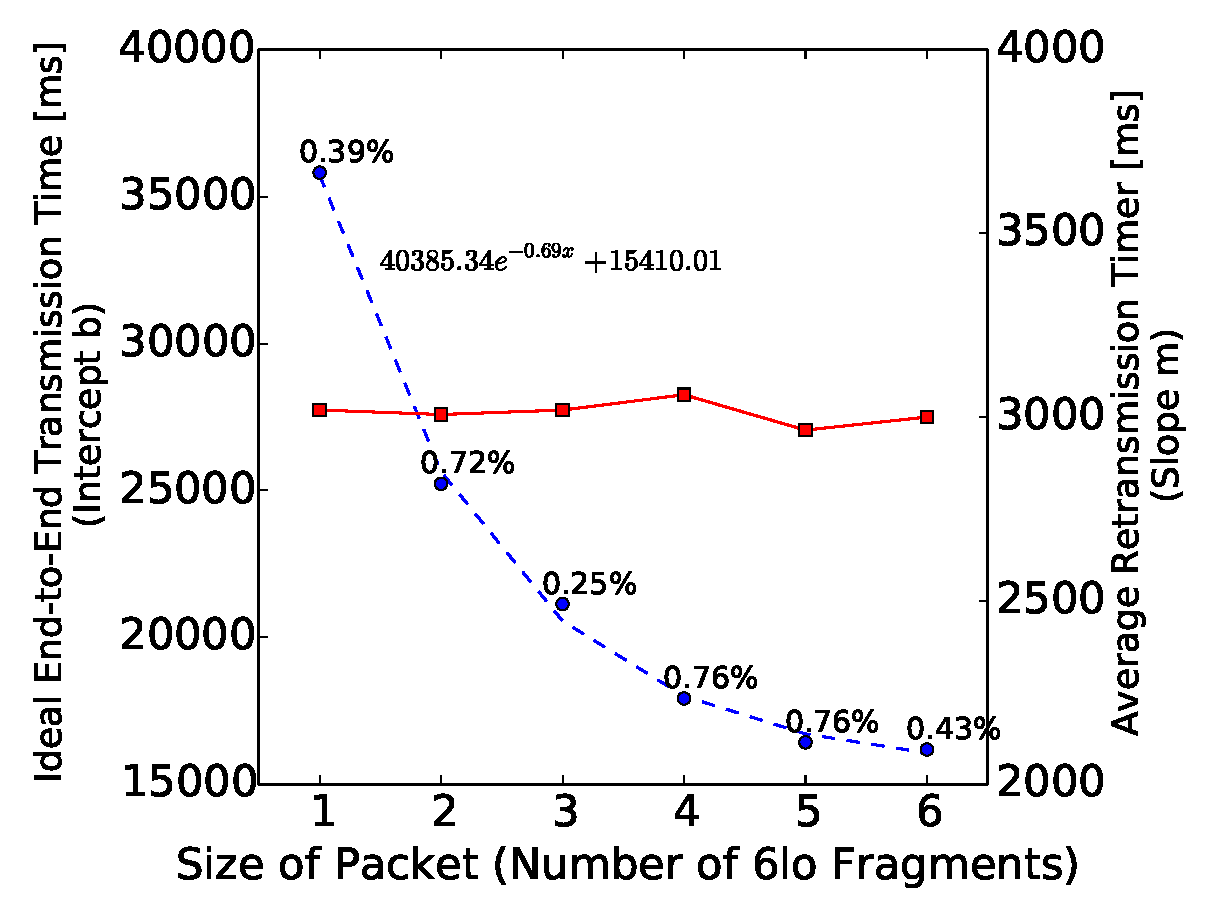
\includegraphics[width=0.5\textwidth]{figs/pa_1}\label{fig:pa1}}
	\subfloat[Linear relationship]{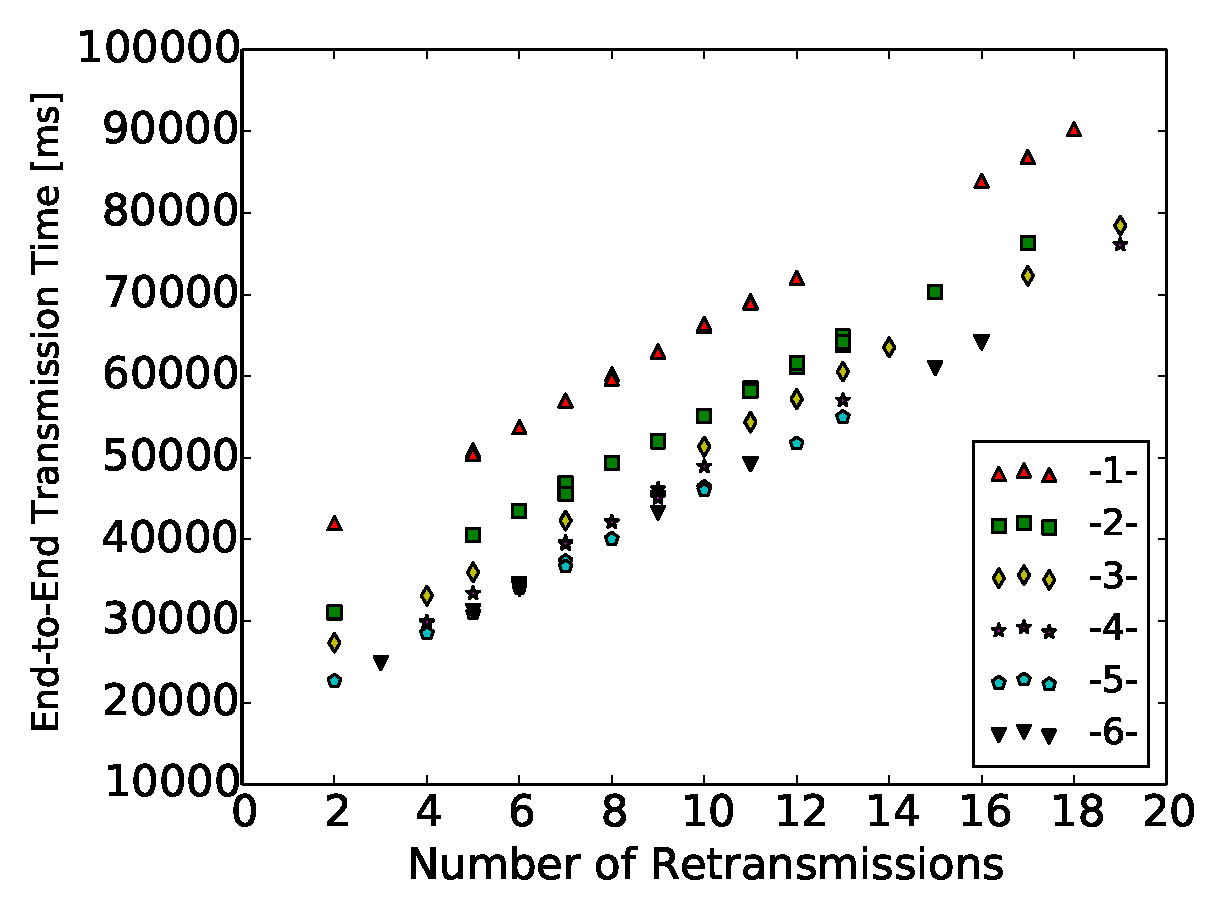
\includegraphics[width=0.5\textwidth]{figs/pa_2}\label{fig:pa2}}
	\caption{Transmitting bulk data (16KiB) in medium traffic (10s) network with link FER(15\%)}
	\label{fig:pa}
	\vspace{-10pt}
\end{figure}
Another function of \emph{Packet Adjustment Module} is to adjust packet size efficiently. When running the experiments in section~\ref{sec:vd}, we find out that there exists a linear relationship between the end-to-end transmission time and the number of retransmissions, as shown in Fig.~\ref{fig:pa2}. For each size of packet we use least squares method to fit the scatters by a linear function $y=mx+b$, and the fitted parameters (slope $m$ and intercept $b$) with normalized root-mean-square deviation (NRMSD) are plotted in Fig.~\ref{fig:pa1}. Both $m$ and $b$ have practical meaning: $m$ is the average value of retransmission timer (3 seconds in our experiments); whereas $b$ implies the end-to-end transmission time in ideal situation where no retransmission occurs. From Fig.~\ref{fig:pa1} it is clear to see that intercept $b$ against the size of packet follows a negative exponential function (dashed line in the figure), which means that the performance gain achievable by increasing packet size is significant when packet size is small; as packet size increases, the gain becomes less significant. With this observation, we set up a threshold value (represented as the number of fragments) in our mechanism. When increasing packet size, if the threshold is not reached, we increase it by one fragment every time; and if the threshold is passed, we increase packet size by its current number of fragments, i.e. doubling the size. Conversely, when decreasing packet size, we half the size if the threshold is not reached; and decrease by one fragment if the threshold is passed.

\section{Evaluation}
We implement our mechanism on Contiki OS and for the configuration of network stack in Contiki, we choose 6lowpan as the adaptation layer and employ CSMA at the link layer to provide media access control. As applications usually require bulk data to be transmitted as soon as possible, we use maximum power to transmit the data. To minimize the latency caused by wake-up synchronization among nodes, we switch \textit{contikimac} to \textit{nullrdc}, in which nodes do not sleep. In practice, nodes can switch back to \textit{contikimac} if necessary after bulk data transmission completes.

\subsection{Simulation Environment}
We simulate a network containing 20 nodes in Cooja, the standard simulator for Contiki. Each node has a transmission range and a larger interference range. Within transmission range, the frame error rate (FER) is able to be configured and it increases as the transmission distance becomes longer; while in interference range, FER is $100\%$ and other nodes are interfered accordingly. We choose one node as the sender (located at one edge of the network) and another node as the receiver (located at the other edge) and there are 4 or 5 hops between the sender and the receiver. Furthermore, to increase simulation fidelity, we generate background traffic in the network by making each node (except the sender and the receiver) send small packets to random nodes randomly within an interval. If the interval is set to 0, then no background traffic is generated.

\subsection{Performance through Large Packets} \label{sec:vd}
In section~\ref{sec:ov} we argued that bulk data transmission in 6lo through large packets can improve network performance significantly. This subsection quantifies this claim. To start with, we establish a medium traffic network (interval is set to 10 seconds) with different FERs ($0\%$, $15\%$, $30\%$, and $45\%$), then transmit the bulk data (16KiB) in different packet sizes. We use two metrics to compare network performance: end-to-end transmission time, and total transmitted octets by all the nodes along the path from the sender to the receiver. We run the tests 20 times for each size of packet. The result from $FER=15\%$ is shown in Fig.~\ref{fig:vd}. Results from other FER values are similar, thus, are omitted for brevity. The exceptional outputs (represented as outliers) are mainly caused by network congestion resulting from the background traffic. Note that the outliers are excluded when calculating the mean value in the figure.
\begin{figure}
	\vspace{-10pt}
	\centering
	\subfloat[End-to-end transmission time (ms)]{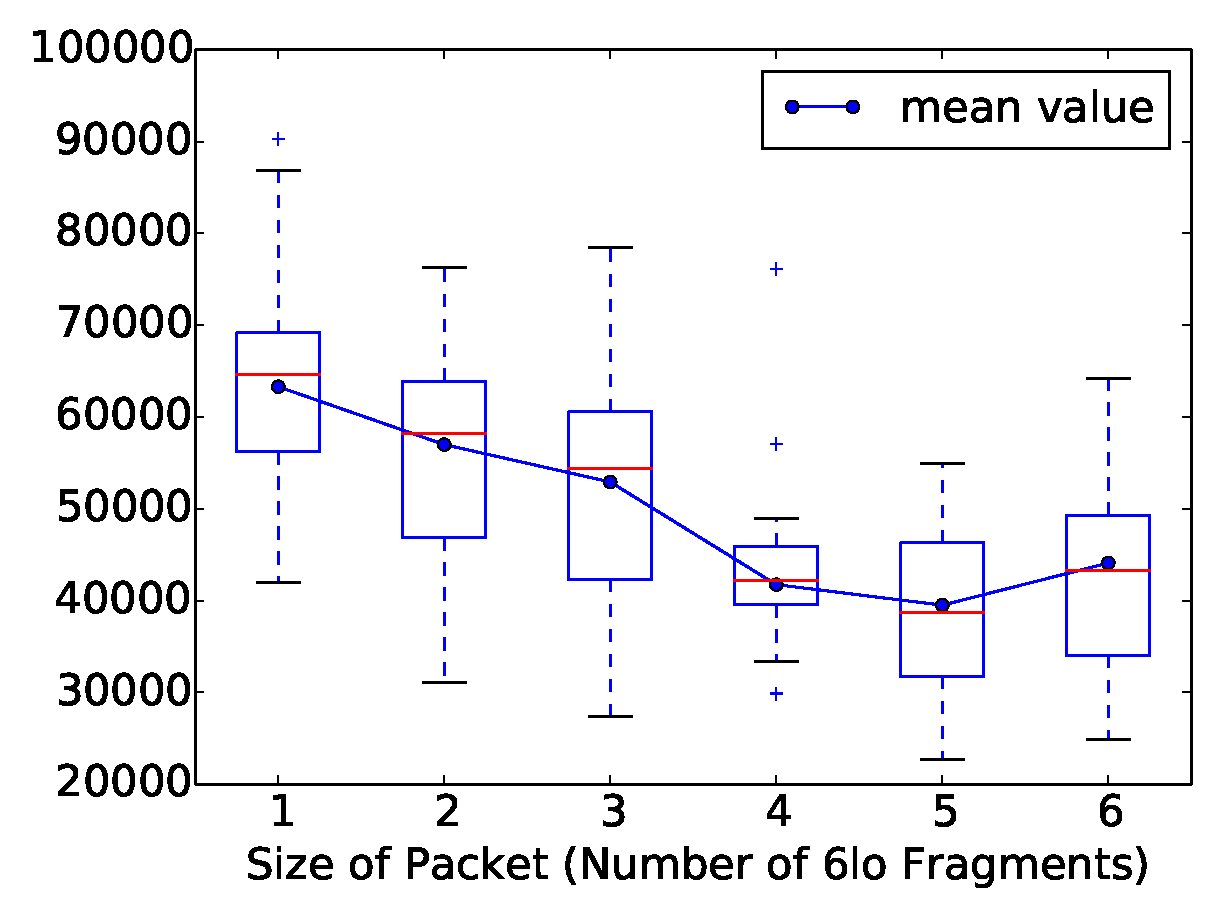
\includegraphics[width=0.5\textwidth]{figs/e2etime}\label{fig:vd1}}
	\subfloat[Total transmitted octets]{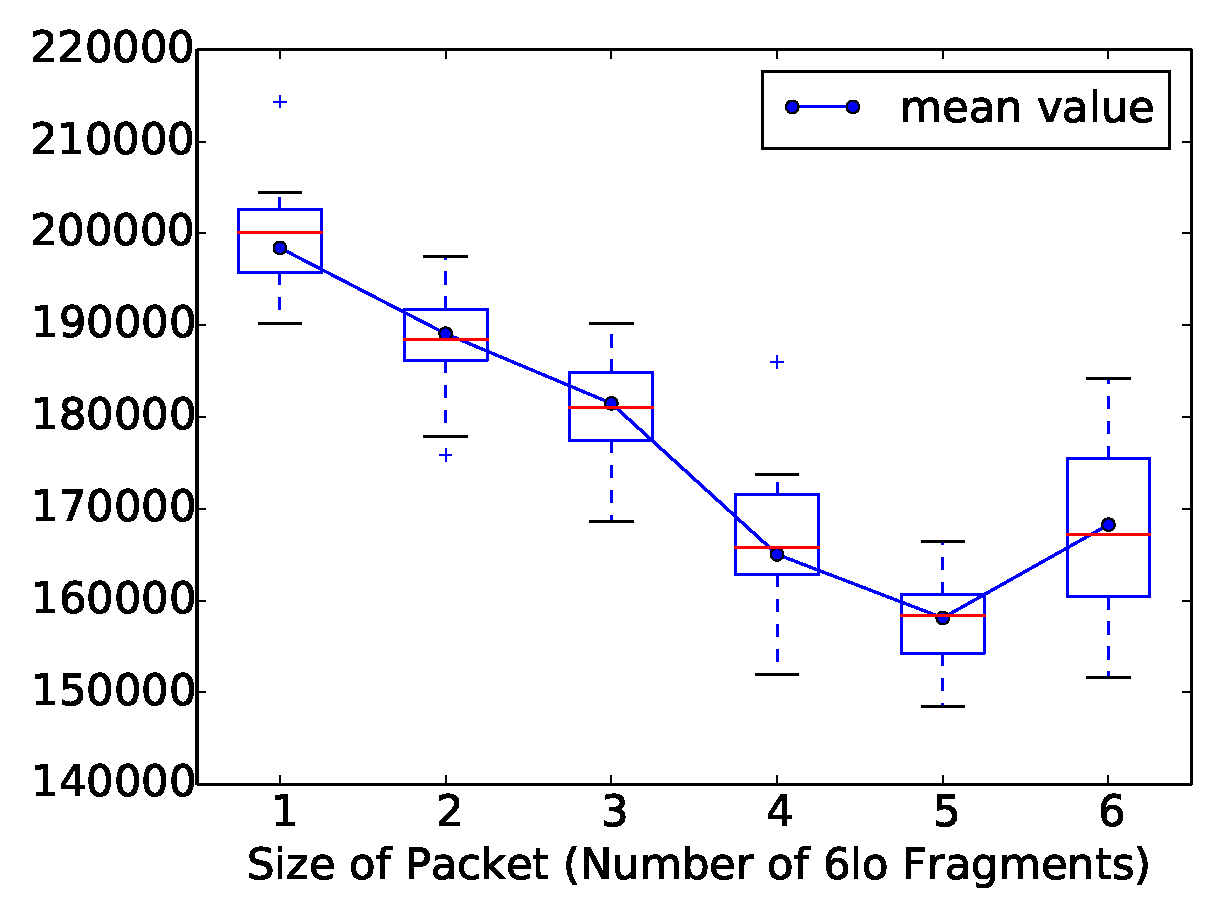
\includegraphics[width=0.5\textwidth]{figs/octets}\label{fig:vd2}}
	\caption{Network performance with $FER=15\%$  for different sizes of packet (represented by number of fragments)}
	\label{fig:vd}
	\vspace{-10pt}
\end{figure}
Fig.~\ref{fig:vd1} illustrates that as the packet size increases the end-to-end transmission time decreases accordingly; however, when the packet size exceeds a specific value, the transmission time increases again. The same trend occurs for the total transmitted octets, as shown in Fig.~\ref{fig:vd2}. The reasons are explained in section~\ref{sec:ov}. From Fig.~\ref{fig:vd}, we can see that if large packets are used, the end-to-end transmission time is improved by $38\%$ (from $\sim 65$s to $\sim 40$s), and total transmitted octets are reduced by $20\%$ (from $\sim 200$KiB to $\sim 160$KiB).

\subsection{Mechanism Effectiveness}
To evaluate the effectiveness of our adaptive mechanism in terms of reliability and goodput, we run a series of experiments in similar simulation environments established in section~\ref{sec:vd} but introducing two more types of background traffic: low traffic (interval is set to 0) and high traffic (interval is set to 5 seconds). Instead of calculating PLR continuously (cf. section~\ref{sec:ov}) to determine network conditions, we simply define network conditions as bad (if retransmission occurs) or good (if the payload is successfully acknowledged). The threshold value introduced in section~\ref{sec:pa} is set to 3, which means that the possible number of fragments is 1, 2, 3, or 6. Bulk data 16KiB is used again and every test runs 20 times.

\begin{figure}
	\vspace{-10pt}
	\centering
	\subfloat[Low traffic]{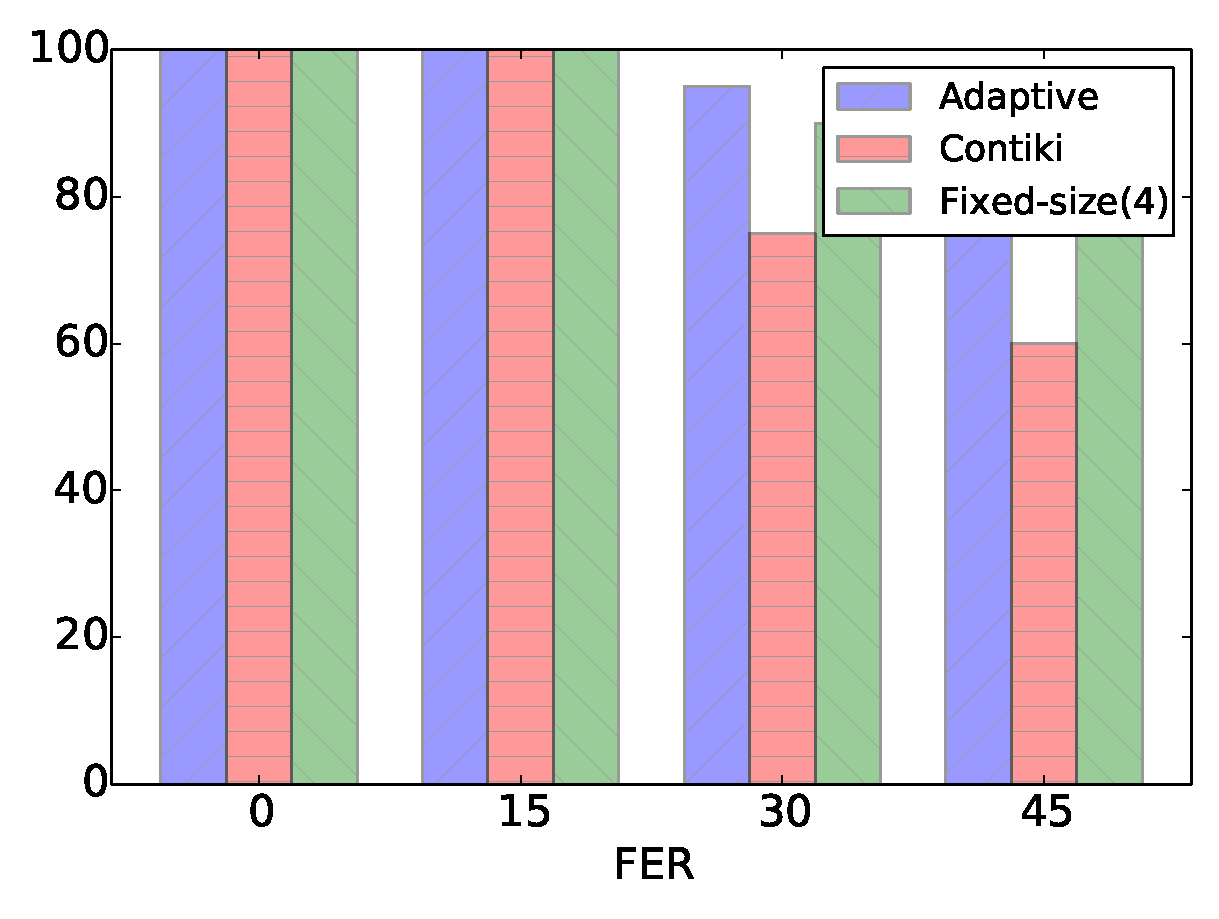
\includegraphics[width=0.33\textwidth]{figs/pct_l}}
	\subfloat[Medium traffic]{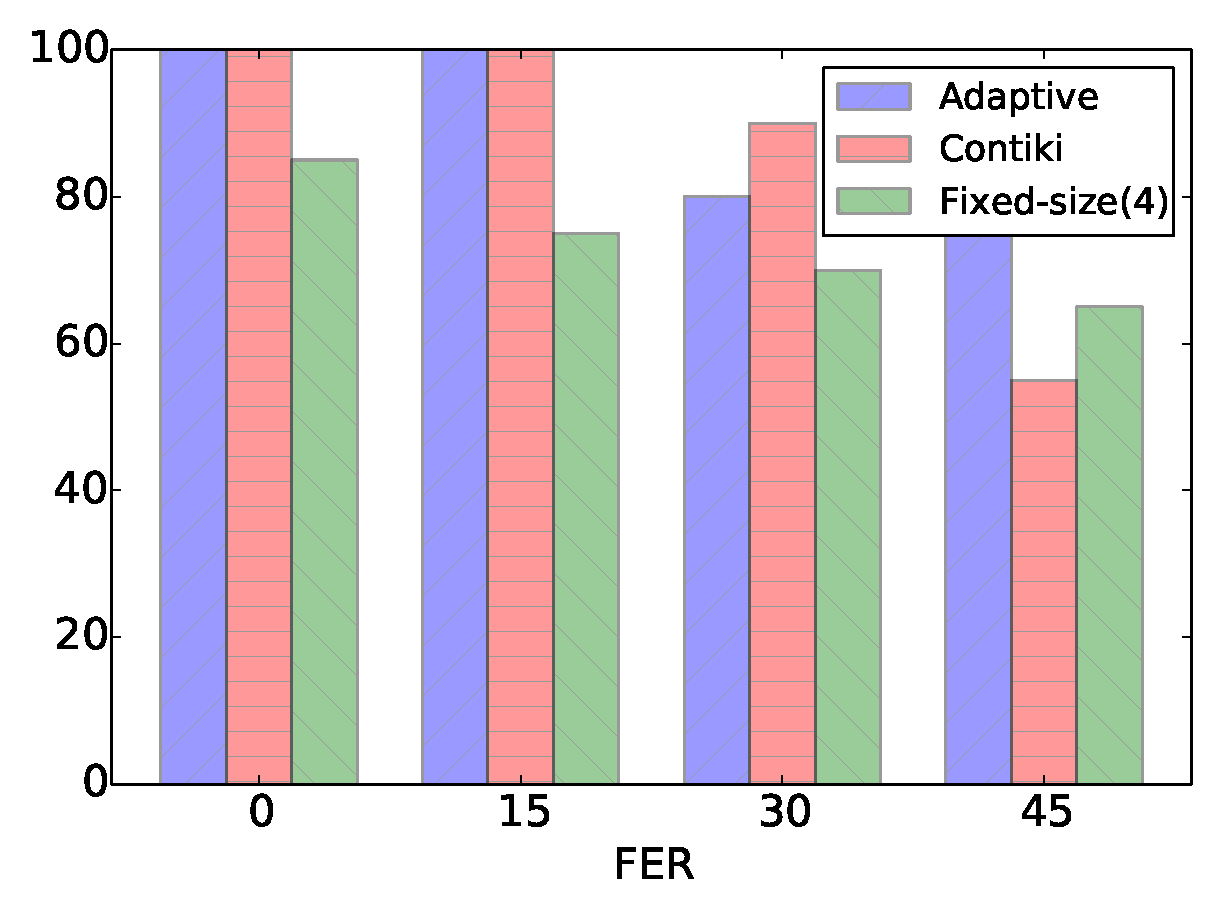
\includegraphics[width=0.33\textwidth]{figs/pct_m}}
	\subfloat[High traffic]{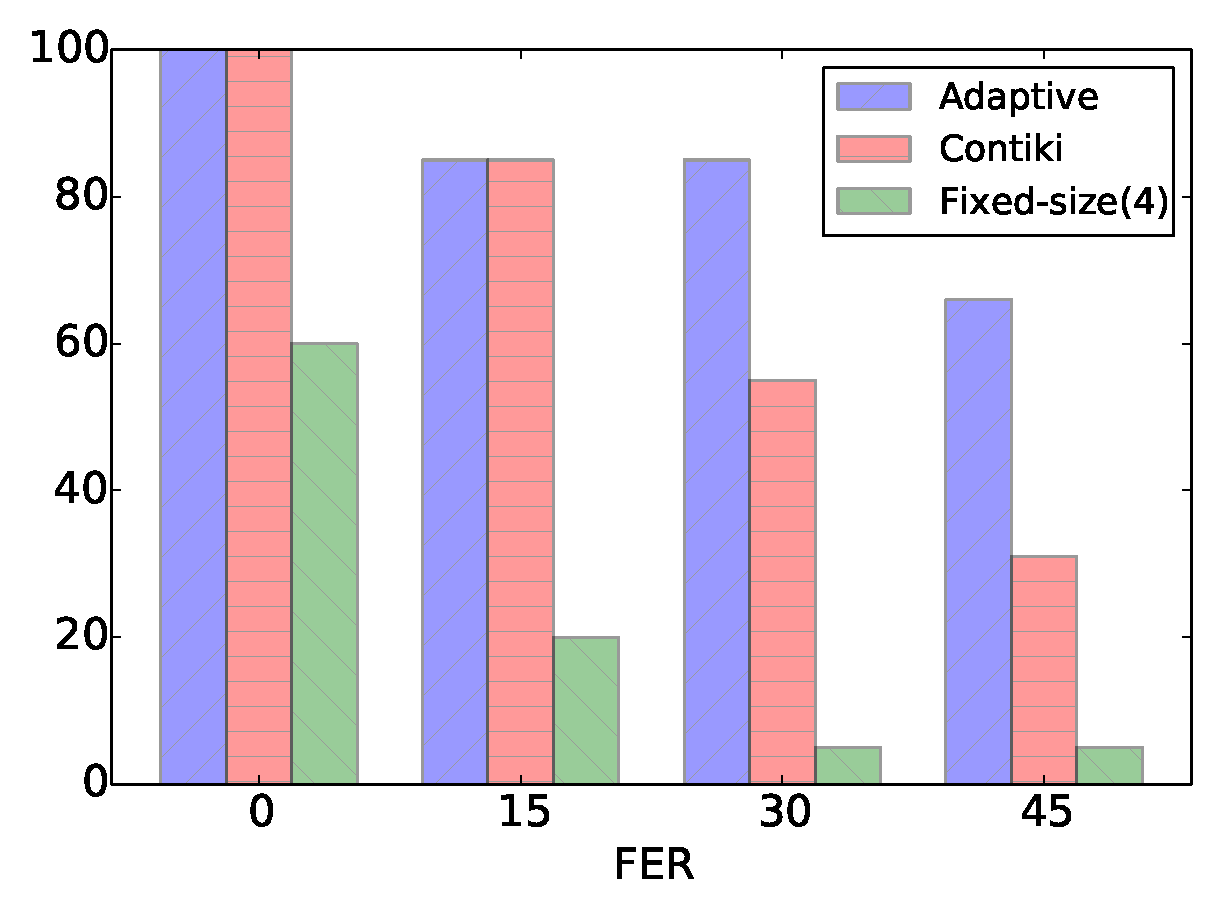
\includegraphics[width=0.33\textwidth]{figs/pct_h}}
	\caption{Percentage of successful transmissions [$\%$], the higher the better.}
	\label{fig:pct}
	\vspace{-10pt}
\end{figure}
We compare our adaptive mechanism (referred to as Adaptive) with the Contiki standard implementation (referred to as Contiki), as well as the approach using a fixed-size packet (referred to as Fixed-size). Firstly, we focus on the percentage of successful transmissions (i.e. how many tests are completed successfully within the 20 tests), which is an indicator of reliability and robustness. The results are shown in Fig.~\ref{fig:pct}. From the figure, we can see that when network traffic is low and link condition is good, all of the three mechanisms complete $100\%$ of tests. When network traffic increases or link condition becomes worse, the percentage of both Adaptive and Contiki decrease slightly, while Fixed-size drops percentage dramatically. We have discussed the reasons for this behaviour in section~\ref{sec:ov}. It is worth mentioning that even in the high network traffic with the worst link condition, Adaptive can still complete around $70\%$ of tests, which is significantly higher than that of Contiki. The reason is that the \emph{Unit Discovery Module} in our mechanism ensures that in the worst cases there is no 6lo fragmentation invoked at any node along the path; while in Contiki, intermediate nodes are still possible to trigger 6lo fragmentation that might lead to packet loss in bad network conditions.

\begin{figure}
	\vspace{-10pt}
	\centering
	\subfloat[Low traffic]{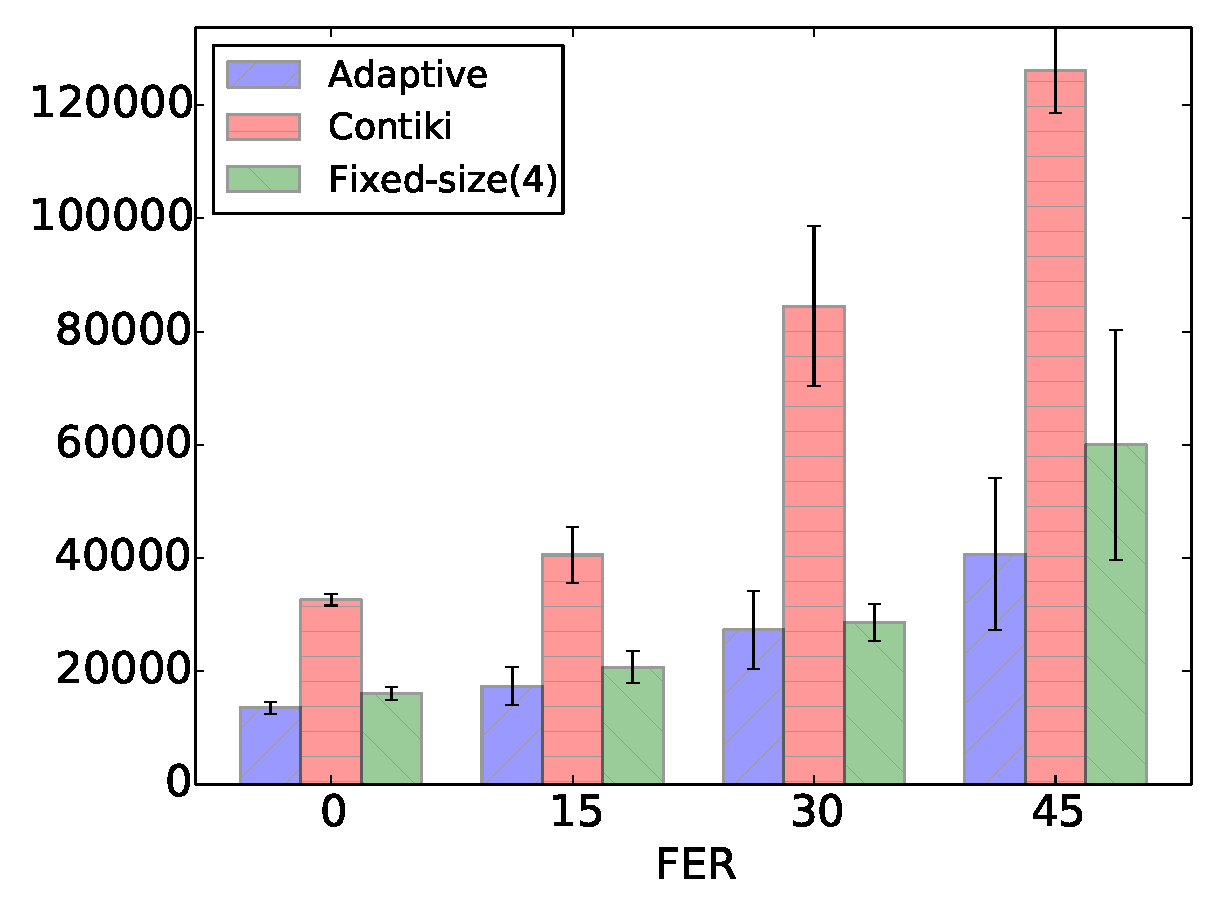
\includegraphics[width=0.33\textwidth]{figs/tm_l}}
	\subfloat[Medium traffic]{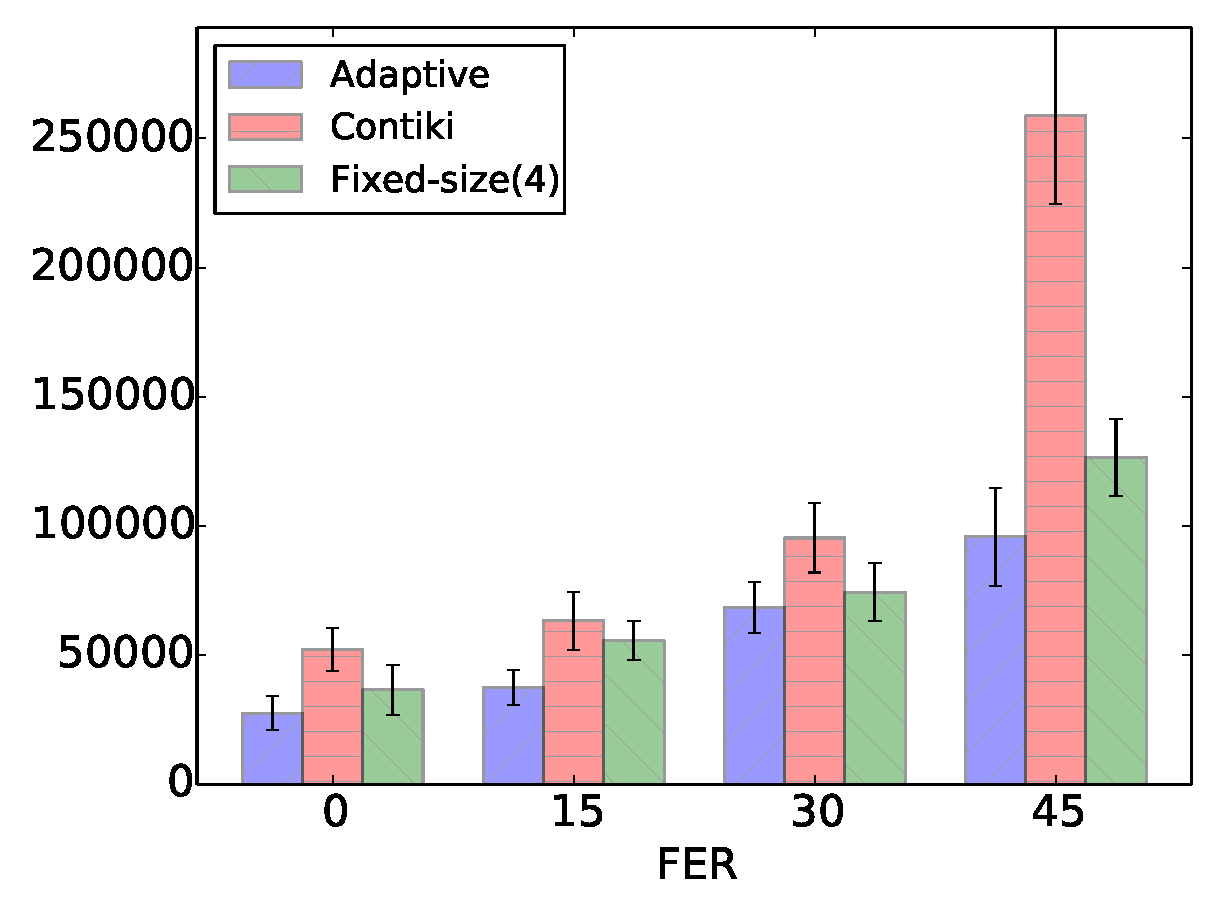
\includegraphics[width=0.33\textwidth]{figs/tm_m}}
	\subfloat[High traffic]{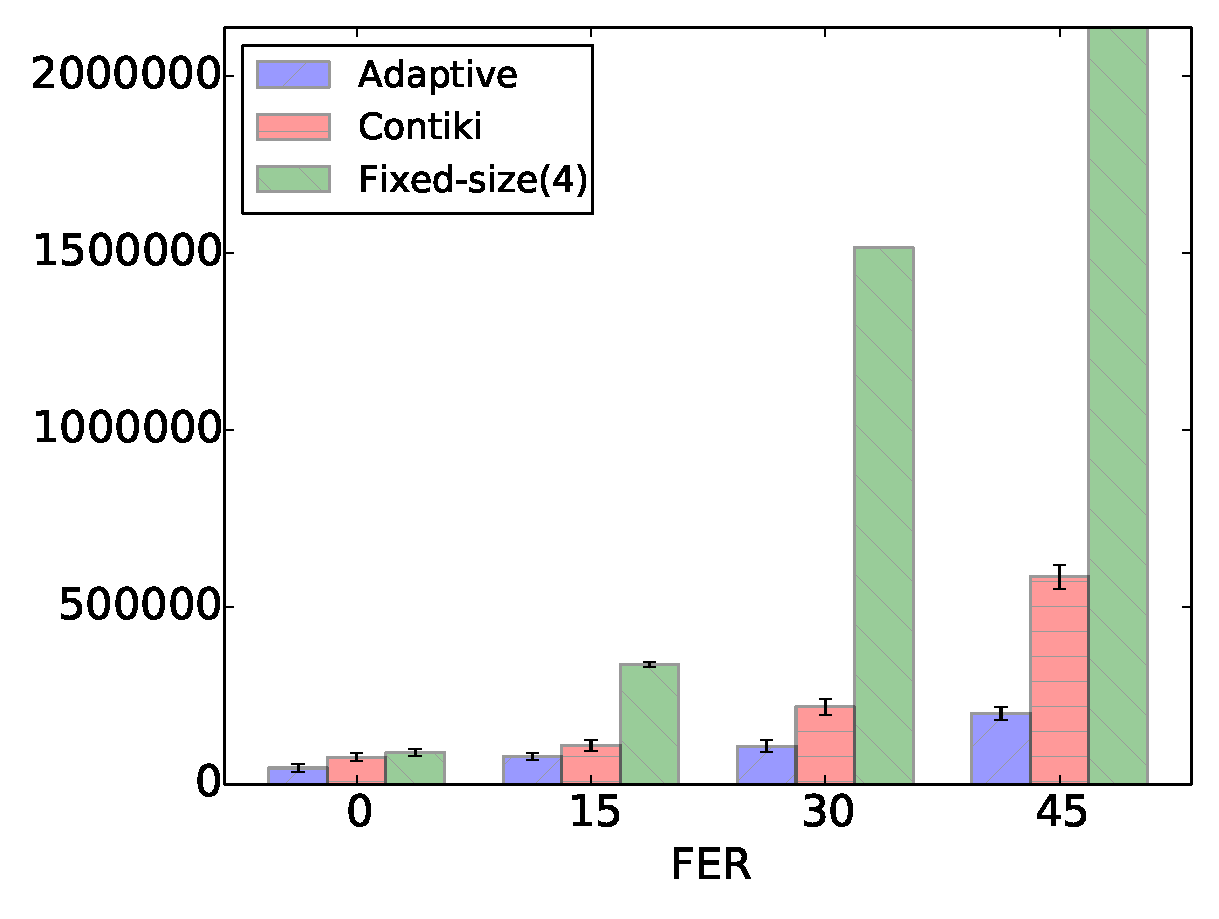
\includegraphics[width=0.33\textwidth]{figs/tm_h}}
	\caption{Estimated end-to-end transmission time [ms], the less the better.}
	\label{fig:tm}
	\vspace{-10pt}
\end{figure}
Secondly, we evaluate network goodput using end-to-end transmission time because network goodput is inversely proportional to end-to-end transmission time. Note that if the test gets failed, it is not possible to acquire the output data. Thus, it is unfair to compare only successful results and exclude the failed cases. To make up for this, we introduce a penalty function, which is defined as $1/percentage$. We then compute the estimated results by successful results times penalty function. We present the estimated results in Fig.~\ref{fig:tm}. From the figure, it is clear that regardless of network traffic, overall transmission time for the three mechanisms increases as link conditions get worse. Compared with Contiki and Fixed-size, Adaptive outperforms them in all three network traffic environments. It is also worth noting that despite the decent performance of Fixed-size for low and medium traffic, the transmission time of it for high traffic is extremely high, which demonstrates its severe weakness in such environments. In summary, our adaptive mechanism is able to provide better reliability and higher goodput than the current state-of-the-art approaches in various network conditions.

\section{Conclusion}
In this paper, we justified the momentum of adaptively adjusting the packet size for bulk data transmission in 6lo. Through an empirical study, we obtained two important observations that inspired the adaptive mechanism directly. By evaluating a series of carefully-designed experiments in Cooja, we demonstrated the effectiveness of our mechanism in term of reliability and goodput. In the future we will conduct a systematic study on real devices. Furthermore, power consumption and duty cycles will also be investigated.

\bibliography{bibtex}
\bibliographystyle{plain}
\end{document}


whose MTU is different, for example, 102 octets for IEEE 802.15.4 without link security, 23 octets for Bluetooth Low Energy, or 128 octets for Near Field Communication by default.

It is worth noting that 6lo fragmentation differs totally from IP fragmentation in that (i) 6lo fragmentation works below IP layer and reassembles 6lo fragments (hereafter referred to as fragments) at the neighbour node whereas IP fragmentation works at IP layer and reassembles IP fragments at the end host; (ii) 6lo fragmentation is allowed to work at routers while IP fragmentation at routers is prohibited strictly by IPv6 specification~\cite{rfc2460} due to harmful issues~\cite{Kent1995}; (iii) 6lo fragmentation saves IP packet overhead but IP fragmentation consumes more as each IP fragment has a header.Other than collaborating with 6lo fragmentation, our mechanism also contains two individual components, namely unit discovery module and packet adjustment module.


We will give a brief mathematical analysis for them in the following:

\emph{Observation 1} can be analysed from two cases. One case is not considering the network traffic then each fragment comprising the large packet is sent in a single frame individually without contention. Thus, PLR is just a function of frame loss rate (FLR) and number of fragments ($N$) $PLR = 1-(1-FLR)^N$, and because FLR is quite small (explained below) $PLR \approx FLR \times N$. The other case is taking the network traffic into consideration then during the period of transmitting fragments there might be other frames competing the channel as well. No matter whether a contention-free beacon mode or a backing-off CSMA algorithm is adopted, the competing frame may be received before all fragments are collected, resulting in failure of packet reassembly. The process of the competing frame ``inserting'' into the fragments can be modelled as a Poisson process whose parameter $\lambda$ reflects the network traffic and parameter $\tau$ is the packet transmission period. We know that the probability of no ``inserted'' frames during packet transmission is computed as $e^{-\lambda\tau}$ so $PLR = 1-e^{-\lambda\tau}$ where $\tau \propto N$. Putting these two cases together, we know that PLR is determined by $N$.

\emph{Observation 2}, given by $PLR \approx FLR \times N$, is the same as FLR is less impacted by the length of frame, which can be explained mathematically as the variance of FLR is quite small when the frame size varies. Because link layer may exploit frame retransmission to improve reliability, $FLR = FER^K$ where $FER$ is the frame error rate and $K$ is the maximum retransmission times. Normally FER is expressed by bit error rate (BER) and frame length ($L$) which is $FER = 1-(1-BER)^L$. And because BER is small, for example the typical value of BER for widely-used Quadrature Phase-shift Keying (QPSK) varies between $10^{-4}$ and $10^{-6}$, $FER$ can be approximately expressed as $FER \approx BER \times L$. By plugging it into FLR formula we get $FLR \approx (BER \times L)^K$. For small-MTU link the value of $L$ is around 100 and the value of $K$ is around 3, therefore FLR is quite small (around $10^{-6}$ for QPSK). Still, because $L$ is relatively small, the variance of FLR would be small too. 


\begin{figure}
	\centering
	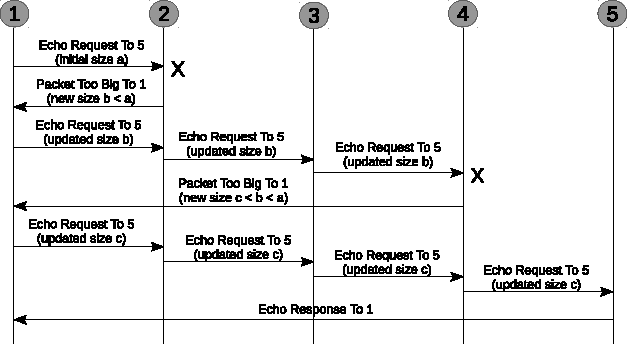
\includegraphics[width=0.7\textwidth]{figs/ud}
	\caption{Unit discovery procedure}
	\label{fig:ud}
	\vspace{-10pt}
\end{figure}

By the definition of unit value, it is trivial to know that if the packet can fit within one single frame (equivalent to one fragment) by all nodes, the size of it should at most be the unit value. Next we think of the cases where the packet is divided into at most two fragments. Considering a packet whose size is just one greater than unit value, still by the definition of unit value we know that there must exists one node that will divide the packet into two fragments. When the packet is to be fragmented, because current frame needs some space to store the initial fragment header and the link MTU is fixed and limited, there must be some octets in the payload unable to be sent within current frame so these octets are left to the second fragment. In addition, the 6lo fragmentation cuts the packet in 8-octet units, which could leave more octets in the payload to the second fragment. Since there are at most two fragments, the second frame is the last frame so it can hold maximum MTU minus non-initial 6lo fragment header. Similarly, we can analyse the cases where the packet is divided into at most $n$ fragments. Then we deduce the following formula to compute the size of packet in octets:


In 6lo many of the link MTUs are quite small comparing to IPv6 minimum MTU (1280 octets), including Bluetooth Low Energy (23 octets), IEEE 802.15.4 (102 octets excluding security), Near Field Communication (128 octets by default), etc. From a networking perspective, not considering the harmful IP fragmentation~\cite{Kent1995}, the link MTU determines the size of IP packet and then determines the ratio of size of IP header to payload (denoted by $ratio$), which is well known to affect the network performance greatly. Thus, in the case of small link MTU if we try to fit each post-compressed IPv6 packet into a single frame, $ratio$ would be relatively large, meaning that more octets have to be sent for equivalent payloads.

Making a comparison of Ethernet and IEEE 802.15.4, $ratio_{Ethernet}=\frac{40}{1500-40}=2.7\%$ while $ratio_{802.15.4}=\frac{7}{102-7}=7.4\%$ is the minimum value and reached when IP header is compressed to 7 octets from 40 octets~\cite{6lowpan2010}. However, best cases take place rarely and for normal cases it would be $ratio_{802.15.4}\approx\frac{13}{102-13}=14.6\%$ approximately.

code overhead and network overhead

optimum value VS our solution

exploring different threshold values